\documentclass[11pt, oneside]{article} 
\usepackage{geometry}
\geometry{letterpaper} 
\usepackage{graphicx}
	
\usepackage{amssymb}
\usepackage{amsmath}
\usepackage{parskip}
\usepackage{color}
\usepackage{hyperref}

\graphicspath{{/Users/telliott_admin/Tex/png/}}
% \begin{center} 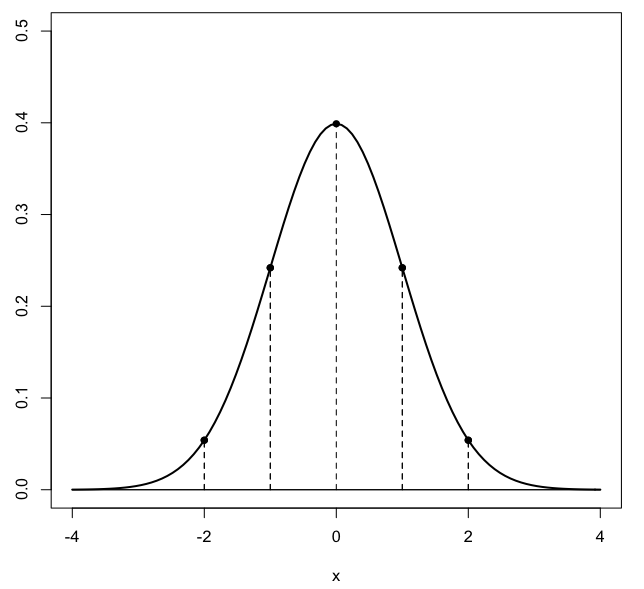
\includegraphics [scale=0.4] {gauss3.png} \end{center}

\title{Easy pieces}
\date{}

\begin{document}
\maketitle
\Large

\subsection*{Integration}
Differentiation breaks things up into small pieces $dx$ or $dr$.  Integration adds up many little pieces.  The symbol for integration is a relaxed S that stands for summation:  $\int$.

As Thompson says
\begin{quote}The word “integral” simply means “the whole.” If you think of the duration of time for one hour, you may (if you like) think of it as cut up into 3600 little bits called seconds. The whole of the 3600 little bits added up together make one hour.\end{quote}

We boldly claim that from the point of view of problem-solving, integration is simply the inverse of differentiation.  

Mathematicians hate this kind of talk, because it trivializes a profound statement, the fundamental theorem of calculus.  

But for practical problem-solving our counter-claim is that this profundity \emph{doesn't matter}.  It is also likely to confuse the beginning student, another reason to put it aside for the time being.  We'll return to this issue later, when we cover the theory of the subject very lightly.

The sum of a bunch of small pieces $dy$ is equal to the sum of a bunch of small pieces $dx$ times $cx$, when $dy/dx= cx$ describes how $y$ changes with small changes in $x$ at any particular point. 

The key idea is \emph{at any point}.  The relationship between $dy$ and $dx$ depends on where you are on the curve.  That's why we need integration.

Write
\[ dy =  f(x) \ dx \]
We want to solve
\[ \int dy = \int f(x) \ dx \]
The sum of all the little pieces $dy$ is just $y$
\[ y = \int f(x) \ dx \]

Now, this surely sounds a little vague.  But it will turn out that
\[ F(x) =  \int f(x) \ dx = y \]

\emph{exactly when} the derivative of $F(x)$ is $f(x)$:
\[ \frac{dF}{dx} = F'(x) = f(x) \]

This is the first of two bright ideas we need to solve an equation like $ \int f(x) \ dx$.  Just find $F(x)$ such that the derivative of $F(x)$ is $f(x)$.

\label{sec:Easy_pieces}

\subsection*{Area of the circle}

Let's spend some time analyzing the area of a circle.  This provides crucial insight into what integral calculus can do.

\begin{center}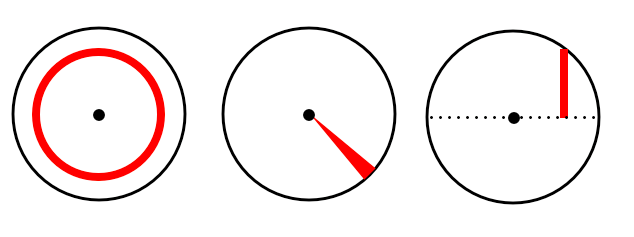
\includegraphics [scale=0.5] {circles3.png}\end{center}

Integration is used to compute areas and volumes, and other sums, by adding up many little pieces.  

To calculate the area of a circle, we find the pieces we will use with one of three basic strategies:  rings, slices of pie, or rectangles of area underneath the function obtained by solving $x^2 + y^2 = R^2$ (using the positive square root).  These three approaches are illustrated in the figure above.

\subsection*{rings}
In the first approach (left panel), we imagine the area being computed by adding up the individual areas of a series of very thin, concentric rings.

The total area to be computed is that of a circle of a definite, fixed size, and we denote the radius of this circle by capital $R$, a constant.  On the other hand, the series of rings ranges from the origin of the circle to the circumference of the outmost ring.  Each one of this progression of rings has a radius, so we use the lowercase $r$ to describe them, with $r$ being a variable---$r$ varies from $0$ at the origin to $R$ at the outside of the circle.

Think about an individual ring, for example the outermost ring, which is similar to the circular peel or rind surrounding a thin slice of lemon.  We are working with areas here, in two dimensions, so the slice we imagine to be infinitely thin, and we are working with it as a cross-section or ring.

The area of the ring is the length times the width.  The length is the circumference, $2 \pi R$ for the outermost ring, but in general, for any of the inner rings it is $2 \pi r$. The length is multiplied by the width of the slice, which is a small element of radius, $dr$.  The small element of area contributed by an individual ring is $dA$:

\[ dA = 2 \pi r \ dr \]

Another way to explain this equation is to ask the question:

\textbf{how does area change with increasing radius}?  

If we take a circle and increase its radius by a little bit, how does the area change?  The answer is, it changes in proportion to the circumference, $2 \pi r$.

Another way to say the same thing is that the derivative is
\[ \frac{dA}{dr} = 2 \pi r \]

Proceeding from the first equation, the total area is the sum of the areas for the series of rings.

\[ A = \int dA = \int_0^R 2 \pi r \ dr \]

It's worth emphasizing how this view is different than the examples of integration one usually sees first in a calculus book:  these pieces of area are not rectangles but circles.  But it poses most clearly the question we are trying to answer, "how does area change as $r$ changes"?

In order to actually determine a value for the area we need two principles.  The first is, as we mentioned before, that the solution to
\[ \int f(x) \ dx \] 
is $F(x)$ if and only if the derivative of $F(x)$ is equal to $f(x)$.

Continuing with our problem
\[ \int 2 \pi r \ dr = 2 \pi \int r \ dr  \]

In this step we used a fundamental rule that a constant can come "out from under" the integral sign.  That's not surprising.  We already know that (at least in the power rule) the derivative of a constant times some function is that constant times the derivative of the function.  We will show that is a general rule later.

Now,  we need to find a function whose derivative is $r$.  
\[ 2 \pi \int r \ dr  \]
We know that function, it is $r^2$, with an extra factor of $1/2$.  
\[ = 2 \pi \ [ \ \frac{1}{2} \ r^2 \ ] \ = \pi r^2  \]

Combining all the coefficients we have $\int 2 \pi r \ dr = \pi r^2$ precisely because the derivative of $\pi r^2$ is just $2 \pi r$.

The second principle we need comes from the Fundamental Theorem of Calculus, which takes account of the bounds on the integral (in this case $0$ and $R$).  The bounds are written attached to the integral as
\[ \int_0^R \]
and on the expression to be evaluated attached to a vertical bar
\[  \bigg|_{r=0}^{r=R} \]
 like this
\[ 2 \pi \int_{r=0}^{r=R}  r \ dr = \pi \ r^2 \ \bigg|_{r=0}^{r=R} \]
We say that the answer is this function, "evaluated between the bounds 0 and R."

The value of such a definite integral is $F(x)$ evaluated at the upper limit minus the value of $F(x)$ evaluated at the lower limit:

\[ = \pi R^2 - \pi (0)^2 = \pi R^2 \]
which appears to be correct.

Note in passing that the lower bound doesn't have to be $0$, it could be some $\rho < R$.  Then we'd have the area of a ring rather than a circle.  And another thing, it's not uncommon to leave out the variable from the bounds, and write it like this:
\[ 2 \pi \int_{0}^{R}  r \ dr \]

\subsection*{wedges}
\begin{center}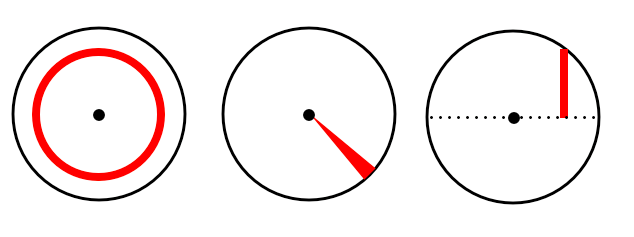
\includegraphics [scale=0.5] {circles3.png}\end{center}
In the second method (middle panel), we need to first find the area of a wedge.  For a thin enough slice, this is a triangle, with a familiar formula: one-half the base times the height.  The height is $R$, the radius of the circle.  

For the base we need the length of a piece of arc of a circle.  Recall that by definition, if we have a unit circle, then the angle of a wedge is equal to the arc it cuts out, and vice-versa, the arc is equal to the angle.  (Thus, the total length if we go all the way around the unit circle is $2 \pi$).  

For a circle with radius $R$, the length going all the way around is $2 \pi R$, and the length of arc for any angle $\theta$ is $\theta$ times $R$.

The area we want is built up of a series of wedges that are almost infinitely slender, with angle $d \theta$, so these wedges have bases measuring $R \ d \theta$.  The area of each triangular wedge is one-half the height times the base or
\[ dA = \frac{1}{2} R \ R \ d\theta \]

For the total area
\[ A = \int dA = \int  \frac{1}{2} R \ R \ d\theta \]
again we see that constants can come outside the integral
\[= \frac{1}{2} R^2 \int_{\theta=0}^{\theta=2\pi} \ d\theta \]
\[ = \frac{1}{2} R^2 \theta \  \bigg|_{\theta=0}^{\theta=2\pi} \]
\[ =  \pi R^2 \]

\subsection*{area under the curve}
\begin{center}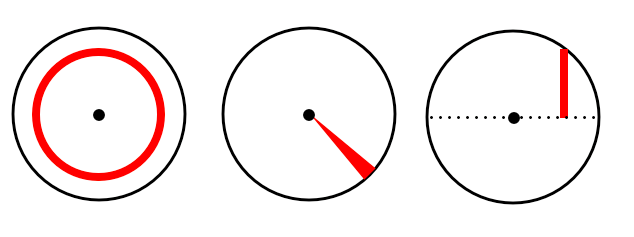
\includegraphics [scale=0.5] {circles3.png}\end{center}

The third view (right panel) is the most familiar, but has a somewhat harder calculation.  We calculate the area under the positive square root in the equation for a circle (right panel), lying above the $x$-axis, and then multiply by two to get the whole thing.
\begin{center}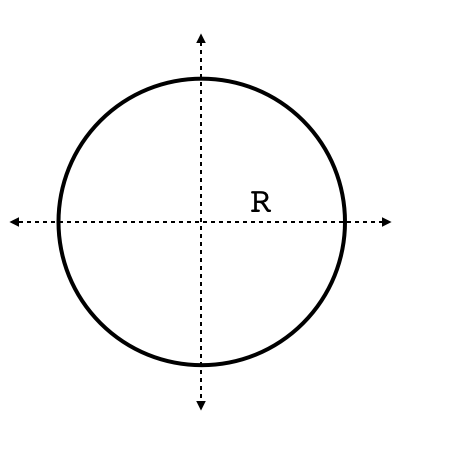
\includegraphics [scale=0.25] {circle.png}\end{center}

\[ x^2 + y^2 = R^2\]
\[ y = f(x) = \sqrt{R^2-x^2} \] 

To get the area, we need to integrate:
\[ \int y \ dx = \int_{-R}^{R} \sqrt{R^2-x^2} \ dx \]

We will work through this problem \hyperref[sec:Cosine_squared]{\textbf{later}}, after we review a few more techniques that are useful in doing integration problems.  

Of course, the answer will turn out to be just what you'd expect.  In fact, this must be so.  If we solve the same problem by correctly using two different techniques and get different answers, then at least one of the techniques is wrong.

The area beneath the circle $y = \sqrt{R^2 - x^2}$ and above the $x$-axis is 

\[ \frac{1}{2} \pi R^2 \]
which is multiplied by $2$ to get the area of the whole circle.

\subsection*{Volume of the sphere}
We think about how the volume of the sphere depends on $r$ ($r = 0 \rightarrow R$).  An incremental change $dr$ changes the volume by adding a thin shell of volume equal to the surface area of the sphere ($4 \pi r^2$) times $dr$.  That is

\[ dV = 4 \pi r^2 \ dr \]
\[ V = \int dV = \int_0^R 4 \pi r^2 \ dr \]
\[ = 4 \pi \ \ \frac{1}{3}r^3 \ \bigg |_0^R = \frac{4}{3}\pi R^3 \]

It's really as simple as that.  Of course, you need to know the formula for the surface area to do it that way.  Alternatively, if you know the volume of the sphere, taking the derivative is an easy way to get a formula for the surface area.

The image shows a "spherical lune", or segment of the surface of the sphere, as an aid to visualizing the whole surface.
\begin{center} 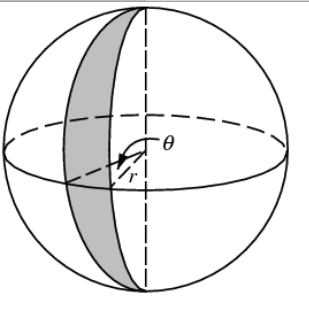
\includegraphics [scale=0.5] {spherical_lune.png} \end{center}
We'll say a lot more about the volume of the sphere \hyperref[sec:Volume_of_the_sphere]{\textbf{later}}. 

\subsection*{technical note}

We should point out that this connection between volume and surface area is not true for \emph{every} solid.  

As an example, the surface area of a cube of side $s$ is $6s^2$, which would have volume $2s^3$ if the relationship were always correct.  In fact, there is something special about the \emph{radial symmetry} of circles and spheres, and their lack of sharp corners and edges.

Here is one more example, to calculate the volume of a cone.  

\subsection*{volume of a cone}

We lay a cone along the $x$-axis with its vertex at the origin, opening to the right.
\begin{center}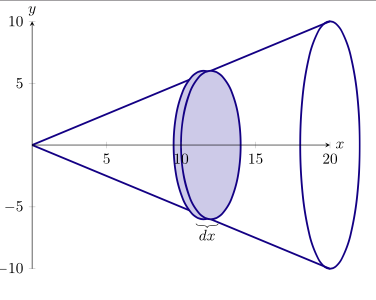
\includegraphics [scale=0.4] {cone_sideways.png}\end{center}
The cone is three-dimensional with the third axis ($z$) coming up out of the page.  The intersection with the $xy$-plane is a triangle.  

Can you see that in the $xy$-plane $y$ is a linear function of $x$, i.e. $y = kx$ where $k$ is a constant.  The constant $k$ is actually the ratio of the radius $R$ to the height $H$.  That is equal to $\Delta y/\Delta x$.
\[ y = \frac{R}{H} x \]

If we slice the cone into thin sections perpendicular to the $x$-axis, each little piece is a circle with radius $y$ and area $\pi y^2$.  For a thin enough slice, the volume is that area times the width of the slice:
\[ dV = \pi y^2 \ dx \]
Finding the volume of an individual piece is the important part of the calculus argument.

Now we just substitute the value of $y$ in terms of $x$
\[ dV = \pi \ [ \frac{R}{H} ]^2  x^2 \ dx \]
add up all the little volumes by setting up the integral
\[ V = \int dV = \int \pi \ [ \frac{R}{H} ]^2 x^2 \ dx \]

We apply the basic rule that constant terms can move "out from under" the integral sign:
\[ = \pi \ [ \frac{R}{H} ]^2 \ \int x^2 \ dx \]
This is a corollary of the result that constants are just carried through in taking the derivative.

We recognize that the value $x$ lies in the interval between $0$ and $H$, $[0,H]$, so these are the "bounds" on the integral, which we write as $\int_0^H$:
\[ = \pi \ [ \frac{R}{H} ]^2 \int_0^H x^2 \ dx \]

and then just follow the rule for doing a problem like this:  $\int x^2 = x^3/3$.  So
\[ = \pi \ [ \frac{R}{H} ]^2 \ [  \frac{x^3}{3} ] \ \bigg |_0^H \]
\[ = \frac{1}{3} \pi R^2 H \]

This is the answer precisely because the derivative of the result ($x^3/3$) is equal to the integrand we started with ($x^2$).

Once again, we obtain the formula of one-third times the area of the base times the height.  No matter what the shape of the base is, the area of each slice will be proportional to $x^2$ and we will end up with a formula involving one-third at the end.

We will see several other methods for obtaining this result.

Note in passing that we can obtain the volume of a fustum (a cone whose top has been cut off) as
\[ = \pi \ [ \frac{R}{H} ]^2 \ [  \frac{x^3}{3} ] \ \bigg |_{h_1}^{h_2} \]
\[ = \pi \ [ \frac{R}{H} ]^2 \ [  \frac{{h_2}^3}{3} -  \frac{{h_1}^3}{3}  \ ] \]

The geometers have given us an even more elegant formula (\hyperref[sec:Frustum]{\textbf{here}}).

\end{document}